\documentclass[fleqn]{article}
\usepackage{graphicx}

\author{jay smith}
\title{HW \#5}
\date{\today}

\begin{document}
\raggedright
\maketitle
\begin{flushleft}


\textbf{Problem \#4}\\

Schematic of circuit with noise sources.
\end{flushleft}

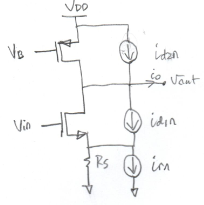
\includegraphics[scale=1.2]{pic1}

\begin{flushleft}
Thermal noise source magnitudes:

\begin{equation}
\overline{i_{d2n}^2} = 4kT\gamma g_{m2}
\end{equation}

\begin{equation}
\overline{i_{d2n}^2} = 4kT\gamma g_{m1}
\end{equation}

\begin{equation}
\overline{i_{d2n}^2} = \frac{4kT}{R_s}
\end{equation}

Solving for iout,n
\begin{comment}

\begin{equation}
i_{0n} = i_{d2n} - i_{d1n} + (\frac{ \frac{1}{g_m1} }{ R_s + \frac{1}{g_m1} }) (i_{d1n} - i_{rn})
\end{equation}


\begin{equation}
i_{0n} = i_{d2n} -  (\frac{ g_{m1}R_s }{ 1 + g_{m1}R_s }) i_{d1n} - (\frac{ 1 }{ 1 + g_{m1} R_s }) i_{rn}
\end{equation}

\begin{equation}
\overline{ i_{0n}^2 } = \overline{ i_{d2n}^2 } + (\frac{ g_{mn}R_s }{ 1 + g_{mn}R_s }) \overline{ i_{d1n}^2 } + (\frac{ 1 }{ 1 + g_{mn}R_s }) \overline{ i_{rn}^2 }
\end{equation}

\begin{equation}
\overline{i_{0n}^2} = 4kT[\gamma g_{mp} + ( \frac{R_s g_{mn} }{ 1+R_s g_{mn} }) \gamma g_{mn} + (\frac{1}{1+g_{mn} R_s}) (1/R_s) ]
\end{equation}

\end{flushleft}
\end{document}